% SECTION : tikz {{{
\section{Tikz}
\label{sec:tikz}
\parindent=0em

\lipsum[1-2]

% tkiz one {{{

\begin{figure}[h!]

% sigmoid  {{{

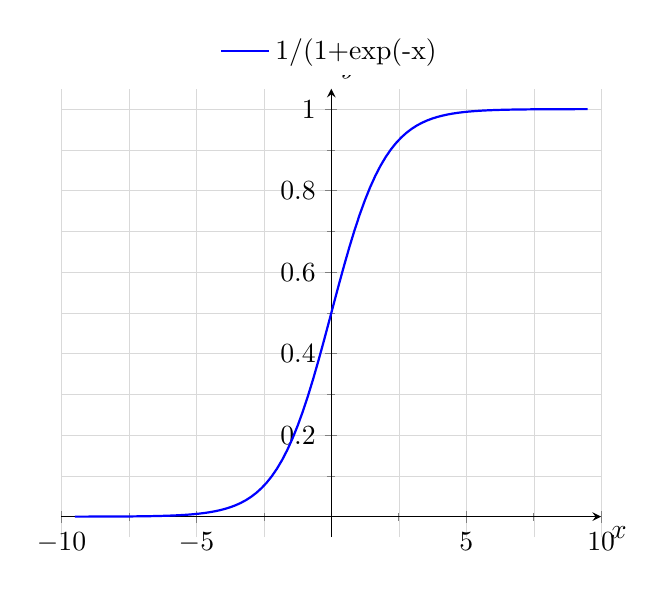
\begin{tikzpicture}
\pgfplotsset{
	every axis legend/.append style={
	at={(0.5,1.03)},
	anchor=south
},
}
\begin{axis}[
%	title          = log(x) / - log(x),
	axis x line    = middle, % x-axis post
	axis y line    = middle, % y-axis post
	minor tick num = 1,      % num axis ticks
    grid           = both,
    grid style     =
	{
		line width=.1pt,
		draw=gray!30
	},
    xmax=10,
    xmin=-10,
    ymin=-0.05,
    ymax=1.05,
	% more plot options in manual for pgfplots
	legend style =
	{
		draw = none % remove legend bounding box
	},
	xlabel       = {$x$},
	ylabel       = {$y$},
    xlabel style =
	{
		at     = {(ticklabel* cs:1)},
		anchor = north west
	},
    ylabel style=
	{
		at     = {(ticklabel* cs:1)},
		anchor = south west
	}
]

\coordinate (O) at (0,0);


\addplot [
	domain=-9.5:9.5,
	samples=100,
	thick,
	blue
]
{1/(1+exp(-x)};
\addlegendentry{1/(1+exp(-x)};

\end{axis}
\end{tikzpicture}

% }}}

\caption{This is a caption.}
\label{fig:placeholder}
\end{figure}
% }}}

\lipsum[1-2]

% tkiz two {{{
\begin{figure}[h!]

% inv log  {{{

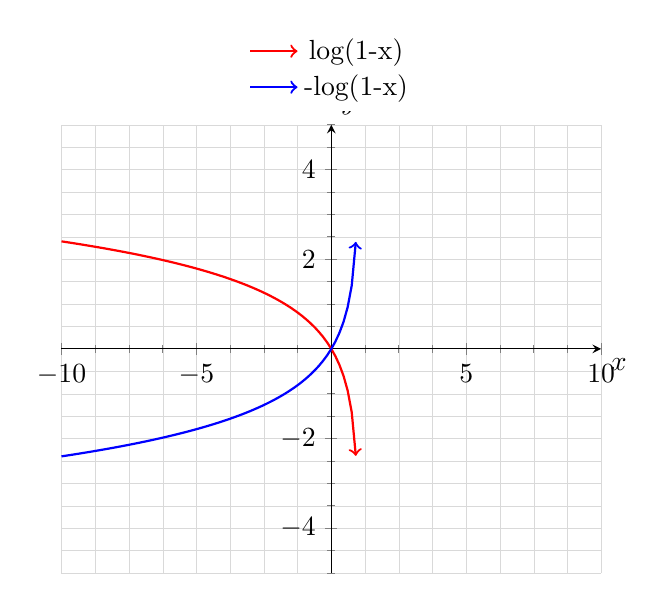
\begin{tikzpicture}

\pgfplotsset{
	every axis legend/.append style={
	at={(0.5,1.03)},
	anchor=south
},
}

\begin{axis}[
%	title          = log(x) / - log(x),
	axis x line    = middle, % x-axis post
	axis y line    = middle, % y-axis post
	minor tick num = 3,      % num axis ticks
    grid           = both,
    grid style     =
	{
		line width=.1pt,
		draw=gray!30
	},
	xmax         = 10,
	xmin         = -10,
	ymin         = -5,
	ymax         = 5,
%	legend pos = outer north east,
	legend style =
	{
		draw = none % remove legend bounding box
	},
	xlabel       = {$x$},
	ylabel       = {$y$},
    xlabel style =
	{
		at     = {(ticklabel* cs:1)},
		anchor = north west
	},
    ylabel style=
	{
		at     = {(ticklabel* cs:1)},
		anchor = south west
	},
]

\coordinate (O) at (0,0);

\addplot
[
	domain=-10:5,
	samples=100,
	thick,
	->,
	red
]
{ln(1-x)};
\addlegendentry{log(1-x)}

\addplot
[
	domain=-10:5,
	samples=100,
	thick,
	->,
	blue
]
{-ln(1-x)};
\addlegendentry{-log(1-x)}


\end{axis}
\end{tikzpicture}

%}}}

\caption{This is a caption.}
\label{fig:placeholder}
\end{figure}
% }}}

\lipsum[3-4]

% page wide tkiz figure {{{

\begin{figure*}[ht]
\centering



\tikzset{basic/.style={draw,fill=blue!50!green!20,text badly centered,minimum width=3em}}
\tikzset{input/.style={basic,circle}}
\tikzset{weights/.style={basic,rectangle,minimum width=2em}}
\tikzset{functions/.style={basic,circle,fill=blue!50!green!20}}


\newcommand{\addsymbol}{\draw[thick] (0.5em,0.5em) -- (0,0.5em) -- (0,-0.5em) --  (-0.5em,-0.5em) (0em,0.75em) -- (0em,-0.75em) (0.75em,0em) -- (-0.75em,0em);}

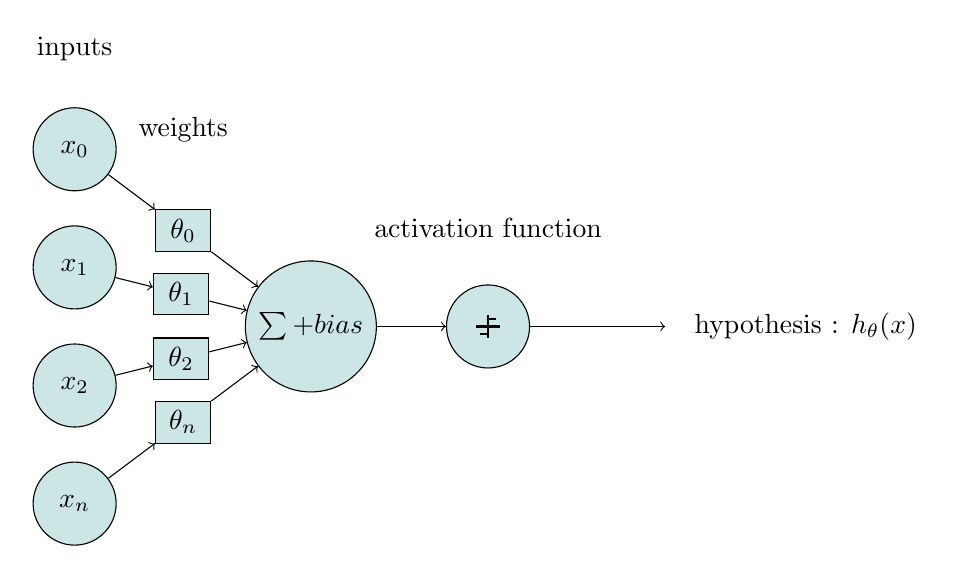
\begin{tikzpicture}[scale=0.75]

\foreach \h [count=\hi ] in {$x_n$,$x_2$,$x_1$,$x_0$}
{
	\node[input] (f\hi) at (0,\hi*2cm-5 cm) {\h};
}

\node[functions] (sum) at (4,0) {$\sum + bias $ };

\foreach \h [count=\hi ] in {$\theta_n$,$\theta_2$,$\theta_1$,$\theta_0$}
{
	\path (f\hi) -- node[weights] (w\hi) {\h} (sum);
	\draw[->] (f\hi) -- (w\hi);
	\draw[->] (w\hi) -- (sum);
}

% show step function symbol
\node[functions] (step) at (7,0) {};
\begin{scope}[xshift=7cm,scale=.75]
	\addsymbol
\end{scope}

\draw[->] (sum)  -- (step);
\draw[->] (step) -- ++(3,0);

% Labels
\node[above=1cm]   at (f4) {inputs};
\node[above=1cm]   at (w4) {weights};
\node[above=1cm]   at (step) {activation function};
\node[right=2.5cm] at (step) {hypothesis : $h_\theta(x)$};

\end{tikzpicture}






\caption{Wide single column figure in a twocolumn document.}
\end{figure*}

% }}}

\lipsum
\lipsum

\sectionend
% }}} END SECTION : tikz

